% Simulating hand-drawn lines with TikZ
% Author: percusse
\documentclass{standalone}
\usepackage{tikz}
\usetikzlibrary{calc,decorations.pathmorphing,patterns}
\pgfdeclaredecoration{penciline}{initial}{
    \state{initial}[width=+\pgfdecoratedinputsegmentremainingdistance,
    auto corner on length=1mm,]{
        \pgfpathcurveto%
        {% From
            \pgfqpoint{\pgfdecoratedinputsegmentremainingdistance}
                      {\pgfdecorationsegmentamplitude}
        }
        {%  Control 1
        \pgfmathrand
        \pgfpointadd{\pgfqpoint{\pgfdecoratedinputsegmentremainingdistance}{0pt}}
                    {\pgfqpoint{-\pgfdecorationsegmentaspect
                     \pgfdecoratedinputsegmentremainingdistance}%
                               {\pgfmathresult\pgfdecorationsegmentamplitude}
                    }
        }
        {%TO 
        \pgfpointadd{\pgfpointdecoratedinputsegmentlast}{\pgfpoint{1pt}{1pt}}
        }
    }
    \state{final}{}
}
\begin{document}
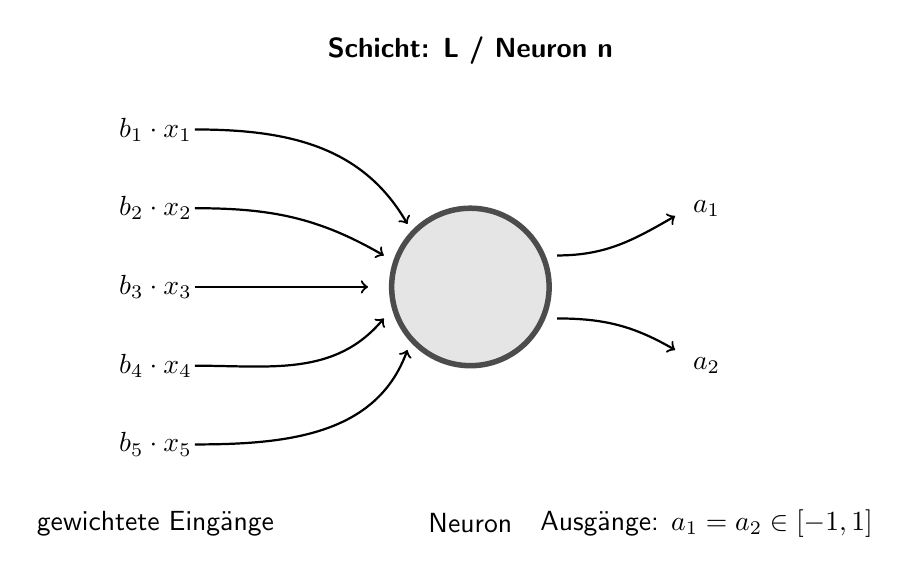
\begin{tikzpicture}[decoration=penciline, decorate, scale=1.0,
    fib masche out/.style={top color=black!80, bottom color=black!80, draw=black!80, rounded corners = 5pt},
    fib masche in/.style={fill=white, draw=white, rounded corners = 5pt},
    fib button out/.style={fill=black!80, draw=black!50},
    fib button in/.style={fill=white, draw=black!50},
    fib electrode/.style={fill=gray!90, draw=white, rounded corners = 5pt},
    fib faeden/.style={fill=gray!80, draw=white, rounded corners = 5pt},
    fib box1/.style={fill=gray!20, draw=black!90, rounded corners = 5pt},
    fib noppen/.style={fill=gray!20, draw=black!70, rounded corners = 5pt, line width=0.07cm},
    fib background vert/.style={left color=black!40, right color=black!10, draw=black!50},
    fib background/.style={fill=black!30, draw=black!50},
    fib lens thick/.style={draw=black!80, line width=0.04cm},
    fib lens thinn/.style={draw=black!95, line width=0.02cm},
    fib mirror/.style={draw=black!60, line width=0.03cm, fill=black!20},
    fib objective/.style={draw=black!60, line width=0.03cm},
    fib quadrupole/.style={draw=black!60, line width=0.03cm},
    fib blanker/.style={draw=black!90, fill=black!60},
    fib octopole/.style={draw=black!80, line width=0.04cm},
  ]
  \draw[fib noppen] (-1,0) circle (1);
\draw
 (-5,2) node[] (vla) {$b_1 \cdot x_1$}
 (-5,1) node[] (vla) {$b_2 \cdot x_2$}
 (-5,0) node[] (vla) {$b_3 \cdot x_3$}
 (-5,-1) node[] (vla) {$b_4 \cdot x_4$}
 (-5,-2) node[] (vla) {$b_5 \cdot x_5$}
(2,1) node[] (vla) {$a_1$}
(2,-1) node[] (vla) {$a_2$}

(2,-3) node[] (vla) {\textsf{Ausg\"{a}nge: $a_1=a_2 \in [-1,1]$}}
(-1,3) node[] (vla) {\textbf{\textsf{Schicht: L / Neuron n}}}
(-1,-3) node[] (vla) {\textsf{Neuron}}
(-5,-3) node[] (vla) {\textsf{gewichtete Eing\"{a}nge}}

;
\path[draw, thick, ->]  (-4.5,2) node[anchor=west] {} to[out=0, in=120] (-1.8,0.8);
\path[draw, thick, ->]  (-4.5,1) node[anchor=west] {} to[out=0, in=150] (-2.1,0.4);
\path[draw, thick, ->]  (-4.5,0) node[anchor=west] {} to[out=0, in=-180] (-2.3,0);
\path[draw, thick, ->]  (-4.5,-1) node[anchor=west] {} to[out=0, in=-130] (-2.1,-0.4);
\path[draw, thick, ->]  (-4.5,-2) node[anchor=west] {} to[out=0, in=-110] (-1.8,-0.8);
\path[draw, thick, ->] (.1,0.4)node[anchor=west] {} to[out=0, in=-150] (1.6,.9);
\path[draw, thick, ->]  (.1,-0.4) node[anchor=west] {} to[out=0, in=150] (1.6,-.8);


%  \draw[decorate,style=help lines] (-0.9,-1) grid[step=1cm] (21.2,11.5);
%%  \draw[decorate,thick] (0,4) -- (14,4);
%%  \draw[decorate,thick] (0,0) -- (14,0);
%  \draw[decorate,thick] (0,6) -- (20,6);
% \draw[decorate,thick] (0,10) -- (20,10);
%
%  \draw[decorate,thick] (20,6) -- (21,7);
%\draw[decorate,thick] (20,10) -- (21,9);
%\draw[decorate,thick] (21,7) -- (21,9);
%
%  \draw[dashed, decorate,thick] (0,0) -- (15,0);
% \draw[dashed,thick] (0,4) -- (15,4);
%  \draw[dashed,decorate,thick] (15,0) -- (20,0);
% \draw[dashed,thick] (15,4) -- (20,4);
%
%  \draw[dashed,decorate,thick] (20,0) -- (21,1);
%\draw[dashed,decorate,thick] (20,4) -- (21,3);
%\draw[dashed,decorate,thick] (21,1) -- (21,3);
%
%
%
%\draw[decorate,thick] (18.5,6) -- (18.5,10);
%\draw[decorate,thick] (15,6) -- (15,10);
%
%%sewing lines
%
%\draw[decorate,thick] (0.5,6-0.25) -- (0.5,6.25);
%\draw[decorate,thick] (0.5,7-0.25) -- (0.5,7.25);
%\draw[decorate,thick] (0.5,8-0.25) -- (0.5,8.25);
%\draw[decorate,thick] (0.5,9-0.25) -- (0.5,9.25);
%\draw[decorate,thick] (0.5,10-0.25) -- (0.5,10.25);
%
%
%\draw[decorate,thick] (1.5,6-0.25) -- (1.5,6.25);
%\draw[decorate,thick] (1.5,7-0.25) -- (1.5,7.25);
%\draw[decorate,thick] (1.5,8-0.25) -- (1.5,8.25);
%\draw[decorate,thick] (1.5,9-0.25) -- (1.5,9.25);
%\draw[decorate,thick] (1.5,10-0.25) -- (1.5,10.25);
%
%
%%\draw[decorate,thick] (15,6-0.25) -- (15,6.25);
%%\draw[decorate,thick] (15,7-0.25) -- (15,7.25);
%%\draw[decorate,thick] (15,8-0.25) -- (15,8.25);
%%\draw[decorate,thick] (15,9-0.25) -- (15,9.25);
%%\draw[decorate,thick] (15,10-0.25) -- (15,10.25);
%%
%%
%%\draw[decorate,thick] (18.5,6-0.25) -- (18.5,6.25);
%%\draw[decorate,thick] (18.5,7-0.25) -- (18.5,7.25);
%%\draw[decorate,thick] (18.5,8-0.25) -- (18.5,8.25);
%%\draw[decorate,thick] (18.5,9-0.25) -- (18.5,9.25);
%%\draw[decorate,thick] (18.5,10-0.25) -- (18.5,10.25);
%%
%%  
%%Masche
%\draw[fib masche out](-0.7,-0.3) rectangle (0,4.3);
%\draw[fib masche in] (-0.55,-0.1)  rectangle (-0.15,4.1); 
%%Masche
%\draw[fib masche out](-0.7,5.7) rectangle (0,10.3);
%\draw[fib masche in] (-0.55,5.9)  rectangle (-0.15,10.1); 
%
%
%%Connect
%\draw[dashed, fib box1] (6.9, 3.1) rectangle (11.7,2.9);
%
%% Toolboxes
%\draw[dashed, fib box1] (3, 0.1) rectangle (7,3.9);
%\draw[dashed, fib box1] (11.5, 0.1) rectangle (13.4,3.91);
%
%\draw[fib electrode](12,0.2) rectangle (12.9,0.8);
%\draw[fib electrode](12,1.2) rectangle (12.9,1.8);
%\draw[fib electrode](12,2.2) rectangle (12.9,2.8);
%\draw[fib electrode](12,3.2) rectangle (12.9,3.8);
%
%%Kletten
%\draw[decorate,thick] (15,6)  -- (18.5,10);
%\draw[decorate,thick] ( 15.8750,6)  -- (18.5,9);
%\draw[decorate,thick] (16.7500 ,6)  -- (18.5,8);
%\draw[decorate,thick] (17.6250 ,6)  -- (18.5,7);
%\draw[decorate,thick] (18.5000 ,6)  -- (18.5,6);
%\draw[decorate,thick] (15,9)  -- (15.8750,10);
%\draw[decorate,thick] (15 ,8)  -- (16.7500,10);
%\draw[decorate,thick] (15 ,7)  -- (17.6250,10);
%
%
%
%  \draw[decorate,thick] (18.5,9) -- (21,9);
%  \draw[decorate,thick] (18.5,9.5) -- (20.5,9.5);
%  \draw[decorate,thick] (18.5,8.5) -- (21,8.5);
%  \draw[decorate,thick] (18.5,8) -- (21,8);
%  \draw[decorate,thick] (18.5,7.5) -- (21,7.5);
%  \draw[decorate,thick] (18.5,7) -- (21,7);
%  \draw[decorate,thick] (18.5,6.5) -- (20.5,6.5);
%
%
%
%
%%Maßstab
%\path[draw,<->, very thick] (19,11)  -- (20,11);
%
%%Beschriftung
%\draw
%(0.3,4.7) node[] (vla) {\underline{\textit{Unterseite}}}
%(0.3,11.2) node[] (vla) { \underline{\textit{Oberseite}}}
%(19.5,10.75) node[] (vla) {\textbf{1cm}}
%;
%
%\path[draw, thick, ->] (9,4.5) node[anchor=west] {fixierte Kabelverbindung} to[out=-180, in=20] (7.5,3.25);
% \path[draw, thick, ->] (14.5,-0.7) node[anchor=west] {starre Silberelektroden} to[out=180, in=-10] (13,0.5);
% \path[draw, thick, ->] (2.5,4.5) node[anchor=west] {Geh\"{a}use: Wearable Kern} to[out=-180, in=180] (2.9,2.9);
% \path[draw, thick, ->] (14.5,4.5) node[anchor=west] {Geh\"{a}use: Elektroden} to[out=180, in=10] (13.5,2.2);
%
% \path[draw, thick, ->] (2.2,5.3) node[anchor=west] {N\"{a}hte} to[out=-180, in=-45] (1.7,6-0.25);
%
% 
% \path[draw, thick, ->] (14.5,10.7) node[anchor=west] {elastisches Material} to[out=-180, in=110] (14,9.5) ;
%
% %\path[draw, thick, ->] (3.5,10.4) node[anchor=west] {Kontakte} to[out=-145, in=0] (1.75,9.25);
%\path[draw, thick, ->] (14.5,5.3) node[anchor=east] {Klett: Schlaufen} to[out=0, in=-90] (16,5.75);
%\path[draw, thick, ->] (19.5,5.3 ) node[anchor=east] {Klett: Widerhaken} to[out=0, in=-90] (20,5.75);
%\path[draw, thick, ->] (1,-0.7)  node[anchor=west] {Spannmasche} to[out=-180, in=-90] (-0.3,-0.5);
%%\path[draw, thick, ->] (4.5,-0.7)  node[anchor=west] {eingen\"{a}hte Silberf\"{a}den} to[out=180, in=-40] (3,.75);
%%\path[draw, thick, ->] (9,-0.7)  node[anchor=west] {Gumminoppen} to[out=180, in=-40]  (7.5,.5);
\end{tikzpicture}
\end{document}